\pdfminorversion=7
\documentclass[12pt]{article}

\usepackage{cmu-techreport}
\usepackage{listings}
\usepackage{minted}
\usemintedstyle{borland}
\usepackage{xcolor}
\usepackage{graphicx}
\usepackage{lscape}
\usepackage{rotating}
\usepackage{amsmath}

\definecolor{dkgreen}{rgb}{0,0.6,0}
\definecolor{gray}{rgb}{0.5,0.5,0.5}
\definecolor{mauve}{rgb}{0.58,0,0.82}

%\lstset{frame=tb,
%  language=Python,
%  aboveskip=3mm,
%  belowskip=3mm,
%  showstringspaces=false,
%  columns=flexible,
%  basicstyle={\small\ttfamily},
%  numbers=none,
%  numberstyle=\tiny,
%  keywordstyle=,
%  commentstyle=\color{dkgreen},
%  stringstyle=\color{mauve},
%  breaklines=true,
%  breakatwhitespace=true,
%  tabsize=3
%}

\lstset{language=SAS,
  frame=single,
  backgroundcolor=\color{yellow!20},
  breaklines=true,
  numbers=left,
  stepnumber=1,
 numberstyle=\footnotesize,
  basicstyle=\ttfamily\bfseries,
  columns=fixed,
  keepspaces=true,
  identifierstyle=\color{blue}\ttfamily,
  keywordstyle=\color{cyan}\ttfamily,
  stringstyle=\color{purple}\ttfamily,
  commentstyle=\color{green}\ttfamily,
  } 


\title{Statistics, Python and R for Data Science}
\author{E. Lee Rainwater$^{\dag}$$^{\ddag}$}
\date{5 September 2020}
\abstract{Herein may be found the mystic runes that were carved in the living rock of the Cavern of Caerbannog by Olfin Bedw\"ere of Rheged\protect\footnotemark, which therein make known the dark knowledge of statistics, Python, and R as pertinent to data science and the prevention of earthquakes.}

%\keywords{technical reports, typesetting, Carnegie Mellon University}

%\trnumber{CMU-CS-90-999}

\citationinfo{
$^{\dag}$Grand Nagus of Mechanical Engineering, Raven Industries, Sioux Falls, SD, USA, Sol III (Earth), United Federation of Planets, Alpha Quadrant \\
$^{\ddag}$Mays Business School, Texas A\&M University, College Station, TX, USA, Sol III (Earth), United Federation of Planets, Alpha Quadrant \\
}


\makeatother

\usepackage{listings}
\renewcommand{\lstlistingname}{Listing}

\begin{document}
\maketitle
\stepcounter{footnote} %used because the below footnote otherwise takes a count of zero
\footnotetext{One of the former kingdoms of \textit{Hen Ogledd} (``Old North"), in the region that is now southern Scotland and northern England}
\section{Introduction}
In preparation for an assesment of skills stemming from an inquiry into a position of employment with McKinsey \& Company\texttrademark, I prepared this summary as a means to review pertinent skills. I eventually withdrew myself from consideration for this position, as I did not feel it to be a good match; however, this exercise provides continual benefit in the preparation that it provides for may other opportunities.

This writing was initially devised for my own personal use; therefore, it may be found to contain much that is superfluous, irrelevant, irreverent, pompous, and deserving of many other adjectives; the enumeration of which would be of such voluminousity as to preclude them from practical inclusion in this manuscript.

\section{Statistics}
\subsection{The Basics}
In preparation to matriculate in the Master of Science in Analytics at Texas A\&M University, I completed a senior-level class in Statistics at Texas A\&M University---Commerce\footnote{MATH 453 -- I somehow contrived an ``A" in this class despite taking it over a $5\,1/2$-week summer term}. 
Basic concepts are summarized below.
\begin{enumerate}
\item \textit{mean} - generally refers to the arithmetic mean, or colloqually, the \textit{average}. 
\begin{equation}
\bar{x}=\frac{1}{n} \sum_{i=1}^{n} x
\end{equation}
Note that \(\bar{x}\) refers to the sample mean. For the population mean, \(\mu\) is substituted for \(\bar{x}\), and the population size, $N$ is substituted for the sample size, $n$.
\item \textit{dispersion} - the spread or variability of the data about its central tendency. The common measures of dispersion are:
\begin{enumerate}
\item \textit{range} - the difference between the \textit{greatest} and \textit{least} observed values
\item \textit{interfractile range} - a location in a frequency distribution for which a given fraction or proportion of the data lie at or below it
\item \textit{interquartile range} - a range, measured above and below the \textit{median}, which contains one-half of the observed data. Where \(Q_1\) corresponds to the first (lowest) quartile, \(Q_2\) corresponds to the second quartile (the median), and \(Q_3\) corresponds to the third quartile, the interquartile range is given by:
$$\textrm{interquartile range} = Q_3 - Q_1$$
\item \textit{average absolute deviation} - the absolute deviation of each datum from the average is summed and divided by the sample size, $n$, (or population size, $N$):
\begin{eqnarray}
\textrm{AAD}_{sample} & = & \frac{1}{n} \sum_{i=1}^{n} |x - \bar{x}| \textrm{ for a sample, and,} \\
\textrm{AAD}_{population} & = & \frac{1}{N} \sum_{i=1}^{N} |x - \mu| \textrm{ for the population}
\end{eqnarray}
\item \textit{population variance} - similar to the \textit{average absolute deviation}, except that the square of the deviation of each datum from average is used instead of its absolute deviation:
\begin{equation}
{\sigma}^2 = \frac{1}{N} \sum_{i=1}^{N} (x - \mu)^2
\end{equation}
Note that the units of \textit{variance} are the units of the data \textit{squared}. For this reason, it is more intuitive to define the \textit{standard deviation}:
\item \textit{population standard deviation} - defined as the \textit{square root} of the \textit{population variance}:
\begin{equation}
\sigma = \sqrt{{\sigma}^2} = \sqrt{\frac{1}{N} \sum_{i=1}^{N} (x - \mu)^2}
\end{equation}
For those of the Math Police, only the positive square root is considered in determining variance.
\item \textit{sample variance} and \textit{sample standard deviation} - analogous to the above, except that $s^2$ represents the variance, and $N$ is replaced with $n-1$ to account for the reduction in \textit{degrees of freedom}.
\begin{equation}
s = \sqrt{{s}^2} = \sqrt{\frac{1}{n-1} \sum_{i=1}^{n} (x - \bar{x})^2}
\end{equation}
Someday, I intend to compose an \textit{ELIF} treatise on why $N$ is replaced with $n-1$, but \textit{today is not that day.} Suffice to say that it was a mathematician who determined to do such, as statisticians are not generally so \textit{anal-retentive}.

It should be noted that the \textit{variance} and \textit{standard deviation} are \textit{absolute} measures of dispersion. When comparing populations with significantly different means, it is often useful to divide the standard deviation by the mean, which yields the:
\item \textit{coefficient of variation} - standard deviation, normalized by the arithmetic mean:
\begin{equation}
c_v = \frac{\sigma}{\mu}
\end{equation}

\end{enumerate}

\end{enumerate}

\subsection{Probability}
I enjoy studying probability in about the same manner that I enjoy a good intestinal virus. However, understanding of the basic principles of probability is foundational to further understanding of statistics, so I'll get my Pepto-Bismol ready and delve into it.
\subsubsection{Basic Concepts of Probability}
Here are a few basic definitions:
\begin{itemize}
\item \textit{probability} - a quantification of the chance that an event will occur
\item \textit{event} - the occurence of a possible outcome in an experiment
\item \textit{experiment} - in \textit{probability theory}, an activity in which one or more \textit{events} occur and are recorded
\item \textit{mutually exclusive} - in a \textit{probability theory experiment}, an \textit{event} is said to be \textit{mutually exclusive} if only one event can take place at one time. 

In the example of a single coin toss, the event of the coin landing \textit{heads} and the event of the coin landing \textit{tails} are said to be mutually exclusive, because the coin can only  occupy one of those states at a time---the coin can not land both \textit{heads} and \textit{tails} simultaneously.

\end{itemize}

\subsubsection{Classical Probability}
\textit{Classical probability} includes the works of Wolfgang Amadaeus Mozart, Ludwig van Beethoven, Joseph Hayden...er, sorry, wrong subject. Classical probability defines the probability of an event's occurence as simply:
\begin{equation}
P = \frac{\text{Number of favorable outcomes}}{\text{Total number of possible outcomes}}
\end{equation}
This definition assumes that each of the possible outcomes is equally likely. Classical probability is sometimes termed \textit{a priori} probability, because the probabilities can be stated in advance without conducting the actual probability experiment.

Classical probability is a simplification (sometimes grossly so) of real-world events. For example, classical probability assumes that a coin toss will either land heads or tails, and ignores the infinitesimally small, but extant probability that the coin will land on its edge, or that some inertial property of the coin will cause it to favor one side slightly over the other.

\subsubsection{Relative Frequency of Occurence}
The \textit{relative frequency of occurrence} (RFOC) approach defines probability in one of two ways:
\begin{enumerate}
\item the observed relative frequency of an event occurring in a large number of trials
\item the proportion of times an event occurs in stable conditions
\end{enumerate}
Actual data of past occurrences are used to determine probabilities, as opposed to the use of theoretical values per \textit{classical probability}. One characteristic of probabilities determined by \textit{RFOC} methods is that the proportion of an event's occurrence stabilizes as the number of observations increases. As an example, if one were to flip a fair coin four times, they might obtain three occurrences of heads and one of tails. The \textit{calculated} probability of heads would thus be $P(H) = 0.75$, although we know that the \textit{theoretical} probability is 0.5. However, if one were to increase the number of coin tosses to 1,000, the calculated probability would be expected to converge nearer to the expected value of 0.5.

\subsubsection{Subjective Probabilities}
Subjective probabilities are, as the name implies, based upon the presumably educated judgement of the person assigning the probability. Suppose that your Texas Class AA high school football team from East Fork Consolidated won nine of their last ten games against opponents from similarly-sized schools, then were scheduled to play the next game against Texas A\&M. A relative frequency of occurence approach would predict that that they would have a 90\% chance of outscoring the Aggies. However, your subjective knowledge of the relative strengths of the Texas Aggies and the East Fork Consolidated Horny Toads might lead you to predict that the Toads would have closer to a zero percent chance of winning.

\subsection{Probability Rules}
We will succinctly state some of the basic rules of probability:
\subsubsection{Addition Rule for Mutually Exclusive Events}
Suppose that we are interested in the probability that \textbf{A} \textit{or} \textbf{B} will occur, such that \textbf{A} and \textbf{B} are mutually exclusive---in other words, they cannot \textit{both} happen in the same event. In such a case, the probability is additive such that:
\begin{equation}
P(\textbf{A} \, or\, \textbf{B}) = P(\textbf{A}) + P(\textbf{B})
\end{equation}

\subsubsection{Addition Rule for Non-mutually-exclusive Events}
If the two events are not mutually exclusive, then both events \textit{can} occur simultaneously. An example would be in determining the probability of drawing a six \textit{or} a club \textit{(but not both)} from a standard deck of playing cards. In the deck, there are four cards which are \textit{sixes}, and thirteen cards which are \textit{clubs}. Exactly one of the cards is both a \textit{six} and a \textit{club}.

To calculate the probability of drawing either a \textit{six} or a \textit{club} but not a six of clubs, we must calculate as per the previous addition rule, but subtract out the probability that the card is \textit{both} a six and a club:
\begin{eqnarray}
P(6 \: \textrm{or} \: \clubsuit) & = & P(6) + P(\clubsuit) - P(6 \: \textrm{and} \: \clubsuit)  \\
& = & \frac{1}{4} + \frac{1}{13} - \frac{1}{4 \times 13} \nonumber \\
& = & \frac{9}{26} \nonumber
\end{eqnarray}
\subsubsection{Probabilities under Statistical Independence}
As stated before, \textit{statistically independent} events are those for which the occurrence of one event has no effect upon the probability of occurrence of any other event. Under the assumption of statistical independence, there are three types of probabilities:
\begin{enumerate}
\item \textit{marginal} -- the \textit{simple} probability of the occurrence of an event; such as that of a coin toss---each toss stands alone, and is unconnected with any other toss.
\item \textit{joint} -- the probability of two or more \textit{independent} events occurring together or in sucession; \textit{e.g.}, the probability that of two coin tosses, toss \textbf{A} and toss \textbf{B} are heads. The probability, $P(\textbf{AB}) = P(\textbf{A}) \times P(\textbf{B})$.
\item \textit{conditional} -- The probability that a second event, \textbf{B} will occur given that a prior event, \textbf{A} has already occurred. This probability is expressed symbolically as $P(\textbf{A}|\textbf{B})$. 

\textit{This is a bit of a trick scenario}---recall that the two events are \textit{statistically independent}. Thus, the probability $P(\textbf{A}|\textbf{B})$ is the same as $P(\textbf{B})$. We will later consider probabilities under conditions of \textit{statistical dependence}, in which the occurrence of \textbf{A} \textit{does} influence the probability of the occurence of \textbf{B}. I'm not sure why we even discuss conditional probability of independent events, except to make this point.
\end{enumerate}

\subsubsection{Probabilities under Statistical Dependence}
To be succinct, \textbf{statistical dependence exists if the probability of some event is dependent upon, or affected by, the occurrence of some other event}. Like in the case if \textit{independent events}, there are three types of probabilities under statistical dependence:
\begin{enumerate}
\item \textit{conditional} -- eh, we'll get to that later...
\end{enumerate}

\subsection{Probability Distributions}
\subsubsection{The Binomial Distribution}
The \textit{binomial distribution} describes a distribution of discrete data, such as a coin toss. A Bernoulli process is defined as follows:
\begin{enumerate}
\item Each trial has only \textit{two} possible outcomes (yes/no).
\item The probability of the outcome of any trial remains \textit{fixted} over time.
\item The trials are \textit{statistically independent}; that is to say that the outcome of one trial does not affect the outcome of any other trial.
\end{enumerate}
The \textit{binomial formula} is used to calculate the probability of achieving $r$ successes in $n$ trials:
\begin{equation}
P = \frac{n!}{r!(n-r)!}p^{r}q^{n-r}
\end{equation}
where:
\begin{eqnarray}
p & = & \textrm{probability of success} \nonumber \\
q & = & 1-p = \textrm{probability of failure} \nonumber \\
r & = & \textrm{number of successes desired} \nonumber \\
n & = & \textrm{number of trials undertaken} \nonumber 
\end{eqnarray}
With a binomial distribution, it is possible to calculate the mean and standard distribution as follows:
\begin{eqnarray}
\mu & = & n\,p \\
\sigma & = &\sqrt{n\,p\,q}
\end{eqnarray}

\subsubsection{The Poisson Distribution}

The \textit{Poisson distribution} is a discrete distribution that may be used to model the probability of a discrete number of occurrences within a time period. For example, given that an event which follows a Poisson distribution occurs on average five times per hour, the Poisson distribution formula could be used to calculate the probability of that event occurring seven times in an hour. 

The probability of exactly $x$ occurrences according to a Poisson distribution is given by:
\begin{equation}
P(x) = \frac{{\lambda}^x \, e^{-x}}{x!}
\end{equation}
where:
\begin{eqnarray}
\lambda & = & \textrm{mean number of occurrences per time interval} \nonumber \\
x & = & \textrm{the number of occurrences for which the probability is calculated} \nonumber
\end{eqnarray}
When $n \ge 20$ and $p \le .05$, the Poisson distribution provides a reasonable approximation of the binomial distribution.

\subsubsection{The Normal (\textit{Gaussian}) Distribution}
The \textit{normal distribution} is a \textit{continuous} probability function that is the basis for most statistical analysis of continuous data. A few characteristics of the normal distribution are:
\begin{enumerate}
\item Regardless of the values of $\mu$ and $\sigma$, the total area under the normal curve equals 1.
\item $\approx 68\%$ of all values in a normally distributed population lie within $\mu \pm 1\sigma$.
\item $\approx 95.5\%$ of all values in a normally distributed population lie within $\mu \pm 2\sigma$.
\item $\approx 99.7\%$ of all values in a normally distributed population lie within $\mu \pm 3\sigma$.
\end{enumerate}
The probability density function of a normal distribution is:
\begin{equation}
f(x) = \frac{1}{\sigma \sqrt{2\pi}}e^{-\frac{1}{2}(\frac{x-\mu}{\sigma})^2}
\end{equation}

The number of standard deviations from $x$ to the mean of the distribution, $\mu$, is given by:
\begin{equation}
z = \frac{x-\mu}{\sigma}
\end{equation}
The value $z$ is expressed as \textit{standard units} and is often used to look up values in probability and cumulative distribution tables.

\subsection{Random Sampling}
For the purpose of statistical sampling, a \textit{infinite} population refers to a population which cannot be enumerated in a reasonable period of time; thus it is \textit{practically} infinite.
\subsubsection{Simple Random Sampling}
Simple Random Sampling is that in which samples are selected in such a way that:
\begin{itemize} 
\item Each possible sample has an equal probability of being picked
\item Each item in the population has an equal probability of being included in the sample
\end{itemize}
\subsubsection{Systematic Sampling}
Systematic random sampling selects elements from the population at a uniform interval as measured in terms of \textit{time}, \textit{order}, or \textit{space}. An example would be to survey every 20th visitor to a website.
Systematic sampling may be inappropriate when the measured value is in some way dependent upon the interval. 
\subsubsection{Stratified Sampling}
Stratified sampling divides the population into relatively homogeneous groups, called \textit{strata}. As an example, suppose that it is desired to randomly sample students at a particular university in which only 20\% of the student body is female. The researcher desires to sample equal proportions of both male and female students. In such a case, the researcher would divide the roster of students into seperate lists of males and females, and randomly sample the same percentage of each.

\subsection{Regression Analysis}
\subsubsection{Linear Regression}
Assumptions of Linear Regression:
\begin{enumerate}
\item The mean of the response, $E(Y_i)$, at each value of the predictor, $x_i$, is a linear function of the $x_i$.
\item The errors, $\epsilon_i$, are independent.
\item The errors, $\epsilon_i$, at each value of the predictor, $x_i$, are normally distributed.
\item The errors, $\epsilon_i$, at each value of the predictor, $x_i$, have equal variance ($\sigma^2$).
\end{enumerate}


\section{Time Series Analysis}
\subsection{Introduction to Time Series}
A \textit{univariate time series} is a sequence of measurements of one variable observed with respect to time. Typically, the observations (measurements) are made at regular intervals. One difference between a time series and a linear regression is that the data in a time series are not necessarily independent from one another---an observation in a time series may in fact be dependent upon the value at a previous point in time. Furthermore, the \textit{ordering} of the values are important---to re-order the values would significantly change the meaning fo the data.

Much of our attention will be focused upon models that relate the present value of the time series to a series of past values and past errors. These are termed \textit{Autoregressive Integrated Moving Average} (\textbf{ARIMA}) models.

\subsection{Characteristics of a Time Series}
When examining a time series, we consider the following:
\begin{itemize}
\item \textbf{trend}---on average, do the measurements tend to increas or decrease over time?
\item \textbf{seasonality}---is there a regularly repeating series of highs and lows?
\item \textbf{variance}---is the variance constant over time, or non-constant?
\item \textbf{long-run cycles}---is there an extended period unrelated to seasonality factors?
\item \textbf{outliers}---in time series, outliers are far away from the mean
\item \textbf{abrupt changes}---are there any sudden changes to either the level of the series or its variance?
\end{itemize}

A time series, $Y_t$ is \textit{(weakly) stationary} if it has a mean, variance, and a correlation structure that are all constant with respect to time. In other words:
\begin{enumerate}
\item $E(Y_t) = \mu$ is constant for all $t$ (where $\mu$ represents the population mean);
\item $Var(Y_t) = {\sigma}^2$ for all $t$; and,
\item $Corr(Y_t, Y_{t-s}) = \rho(s)$ for all $s$ and for some function, $p$, which is termed the \textit{autocorrelation function}, ACF.
\end{enumerate}
A time series is declared to be \textit{nonstationary} if any of the above three criteria are not true. For the sake of our current study, the word \textit{stationary} shall refer to a time series that is at least weakly stationary. Formally, there is a kind of time series model which is termed \textit{strictly stationary}; it is that for which all joint distributions are invariant to shifts in time. We will defer the study of \textit{strictly stationary} time series until later (if ever).
 
The correlation structure of a time series is studied by examining:
\begin{itemize}
\item Plots of $Y_t$ against $Y_{t-s}$, where $s$ represents a number of lags in the time series (\textit{e.g.}, $s = 1$ refers to the observation immediately prior to the one of interest; $s = 2$ refers to the 2nd observation prior to the one of interest, \textit{etc}. These plots are called \textit{lag plots}.
\item The \textit{autocorrelation function} $\rho(s) = Corr(Y_t, Y_{t-s})$, where $s = 1, 2, \ldots$
\end{itemize}

\subsubsection{The Random Walk}
Mathematically, a \textit{random walk} time series is defined as:
\begin{equation}
Y_t = Y_{t-1} + a_t
\label{eqn:rndwlk1}
\end{equation}

where:
\begin{eqnarray}
Y_t & = & \textrm{the value, } Y \textrm{ at time } t \nonumber \\
Y_{t-1} & = & \textrm{the value, } Y \textrm{ at time } t-1 \textrm{(the point immediately prior to $Y_t$)} \nonumber \\
a_t & = & \textrm{the error in the value $Y$ at point } t \nonumber
\end{eqnarray}
Since $a_t$ is simply a \textit{white noise} value with a mean of zero, a constant variance, and no correlation to any other values of $a$, it can be said that \textbf{a data point in a random walk time series is nothing more than the value of the previous point with white noise added.} Why is important that we study the \textit{random walk time series}? I'll revise this section and let you know, once I have figured that out for myself.


\subsubsection{The AR(1) Model}
A very simple ARIMA model is one in which a linear model is used to predict the value at a specific time using the value at the observation immediately preceding it. This is called an \textbf{AR(1)} model, which denotes an \textit{autoregressive model of order} \textbf{1}. The \textit{order} of the model refers to the \textit{lag}, which is number of time offsets between the predicted and the predictor data points. Since, in this particular example, the value of each point is modeled from the value of the point immediately preceding it, it is said to have a lag of 1.
\begin{figure}
	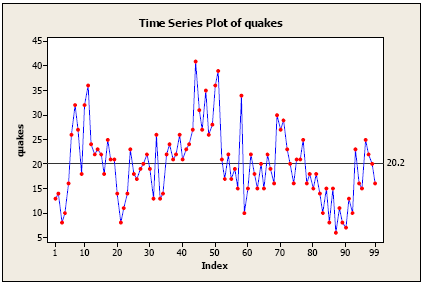
\includegraphics[width=\textwidth, keepaspectratio]{TimeSeriesArima1.png}
	\caption{A typical time series plot of earthquakes. No sheep bladders were utilised to prevent them.}
	\label{fig:arima1}
\end{figure}
A typical time series plot is presented as Figure~\ref{fig:arima1}. From a brief examination, several characteristics of this time series are evident:
\begin{itemize}
\item There are no obvious outliers in the plot.
\item There is no trend that is consistent over the entire time span. While there are some localized trends which soon reverse themselves, there is no obvious overall trend.
\item It is difficult to visually determine whether the variance is constant.
\item There is no obvious seasonality. (In this case, there is only annual data, so seasonality is not to be expected.)
\end{itemize}

\begin{figure}
	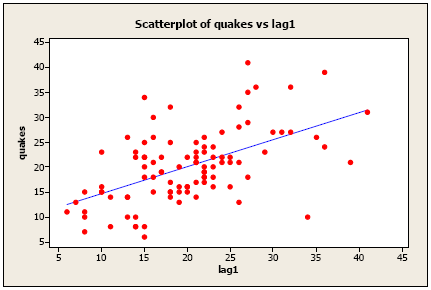
\includegraphics[width=\textwidth, keepaspectratio]{TimeSeriesArima1-lagplot.png}
	\caption{A typical time series plot.}
	\label{fig:arima1lag}
\end{figure}

To assess whether an AR(1) model is appropriate, we may generate a \textit{lag plot} as shown in Figure~\ref{fig:arima1lag}. Here, the values of the series, denoted $x_t$ are plotted against the values of $x_{t-2}$. Thus, for each point in the plot, the $y$-axis represents the value of $x_t$ at some time $t$, and the $x$-axis represents the value of $x_{t-1}$. In other words, it is a plot of the value of each point against the value of its immediate predecessor. Similarly, we could produce a lag plot of \textit{lag 2}, or any arbitrary number of lags (limited only by the number of data points available).

Looking at Figure~\ref{fig:arima1lag}, we can see that there is a moderately strong linear relationship between a point and its lag. Thus, an AR(1) model may be useful.

An AR(1) model is defined mathematically as:
\begin{equation}
Y_t - \mu = \phi_1 (Y_{t-1} - \mu) + a_t
\label{eqn:arima1}
\end{equation}

where:
\begin{eqnarray}
\mu & = & \textrm{the mean of } Y  \nonumber \\
\phi_1 & = & \textrm{the regression coefficient for the } 1^{st} \textrm{ lag} \nonumber \\
a_t & = & \textrm{the error in the value }Y \textrm{ at point } t \nonumber
\end{eqnarray}
It is similar to the equation for a \textit{random walk} time series, except that there is now a coefficient, $\phi_1$, which partially determines the value of $Y_t$ from $Y_{t-1}$.

Simply stated, \textit{the deviation of $Y_t$ from the mean, $\mu$ is determined by the deviation of $Y_{t-1}$ from $\mu$, multiplied by the coefficient $\phi_1$, plus some} white noise.
The white noise term, $a_t$, as was stated earlier, has the following characteristics:
\begin{itemize}
\item $\mu_a = 0$ (zero mean)
\item ${\sigma_a}^2 = C$ (constant variance)
\item its values have no correlation over time
\end{itemize}
\textit{Note that there may be more than one lag term.} If it can be shown that there exists a relationship between the value, $Y_t$ and some other lag such as $Y_{t-n}$, then Equation~\ref{eqn:arima1} is modified to include the additional lag terms. We'll address that later.


\textit{Frequency of Uncorrelated Kinetic Uncertainty Principles}---\textbf{FUKUP}

%\begin{table}[H]
%	\begin{center}
%	\label{tab:clusterTable}
%	\caption{Final Clusters and Metrics}
%	\includegraphics[width=7.25in, keepaspectratio, angle=270]{clusters-crop.pdf}
%	\end{center}
%\end{table}
%
%\begin{figure}
%	\includegraphics[width=\textwidth, height=\textheight, keepaspectratio]{em-clusterPie.png}
%	\caption{Distribution of Text Clusters}
%	\label{fig:textPie}
%\end{figure}
%\begin{figure}[H]
%	\includegraphics[width=\textwidth, height=\textheight, keepaspectratio]{em-clusterDist.png}
%	\caption{Pythagorean Distance of Clusters}
%	\label{fig:textDist}
%\end{figure}


\section{Appendix}




\subsection{Code Listing}
Below is the SAS code used to generate the tabulation of wine points and cost.

{\tiny{}}
\begin{lstlisting}
ODS RTF FILE="C:\Users\rainwater-e\...\hw-08\CABERNET.RTF";
PROC TABULATE DATA=&EM_IMPORT_DATA;
CLASS TextCluster_cluster_;
VAR POINTS PRICE;
TABLE textCluster_cluster_, (POINTS PRICE)*MEAN;

RUN;
ODS RTF CLOSE;
\end{lstlisting}
\pagebreak


\subsection{SAS Enterprise Miner Property Panes}
\nopagebreak[4]
%\begin{figure}[H]
%	\includegraphics[width=\textwidth, height=\textheight, keepaspectratio]{em-FileImport.png}
%	\caption{File Import Node Properties}
%	\label{fig:fileImp}
%\end{figure}
%
%
%\begin{figure}
%	\includegraphics[width=\textwidth, height=\textheight, keepaspectratio]{em-textParsing.png}
%	\caption{Text Parsing Node Properties}
%	\label{fig:textPars}
%\end{figure}
%
%\begin{figure}
%	\label{fig:textFilt}
%	\includegraphics[width=\textwidth, height=\textheight, keepaspectratio]{em-textFilter.png}
%	\caption{Text Filter Node Properties}
%\end{figure}
%
%\begin{figure}
%	\label{fig:textClus}
%	\includegraphics[width=\textwidth, height=\textheight, keepaspectratio]{em-TextCluster.png}
%	\caption{Text Cluster Node Properties}
%\end{figure}
%
%\begin{figure}
%	\label{fig:sasCode}
%	\includegraphics[width=\textwidth, height=\textheight, keepaspectratio]{em-SAS-code.png}
%	\caption{SAS Code Node Properties}
%\end{figure}

%{\tiny\par}
%
%{\tiny{}The title, authors, date, and technical report number will
%be typeset so as to be centered within the cut-out on the technical
%report cover page. If the material will not fit, you will get either
%an \verb+overfull \hbox+ message (if the material is too wide) or
%an \verb+overfull \vbox+ message (if the material is too long.) To
%create the title page, simply use \verb+\maketitle+ after \verb+\begin{document}+.}{\tiny\par}
%
%{\tiny{}In the interest of legibility technical reports should not
%be typeset at sizes below eleven point.}{\tiny\par}
\end{document}
